\section{Data} \label{sec:data}

In this section we will describe the dataset we have worked with, how we
partitioned the dataset into pieces (train, validation, test), the preprocessing
steps we applied to the dataset, the reasons behind those preprocessing steps,
and how we generated problem instances to train our neural networks on.


\subsection{Data Split}

Our dataset is provided by the Danish company MaCom. The dataset is a file
consisting of a set of texts written in Danish where each text is associated
with an author ID. Throughout the development process we have been given
several data extracts. We will only discuss the last dataset as the other are
irrelevant. The texts in the dataset is extracted from pdf files meaning that
sometimes the texts are not valid texts. The final extract consisted of a set of
10,058 authors where a maximum of 100 authors were extracted from each school.
In total the dataset contains 133,749 texts. We needed to split the dataset into
pieces as we needed several different datasets for different purposes in our
experiments. The split is illustrated in Figure \ref{fig:data_split}. Each split
is performed on the author level such that if a single text $t \in T_\alpha$ is
in a particular dataset then all $t' \in T_\alpha$ is in that same dataset. We
have named our datasets as upper case characters. The different datasets we use
are,

\begin{figure}
    \centering
    \textbf{Dataset Partition}\par\medskip
    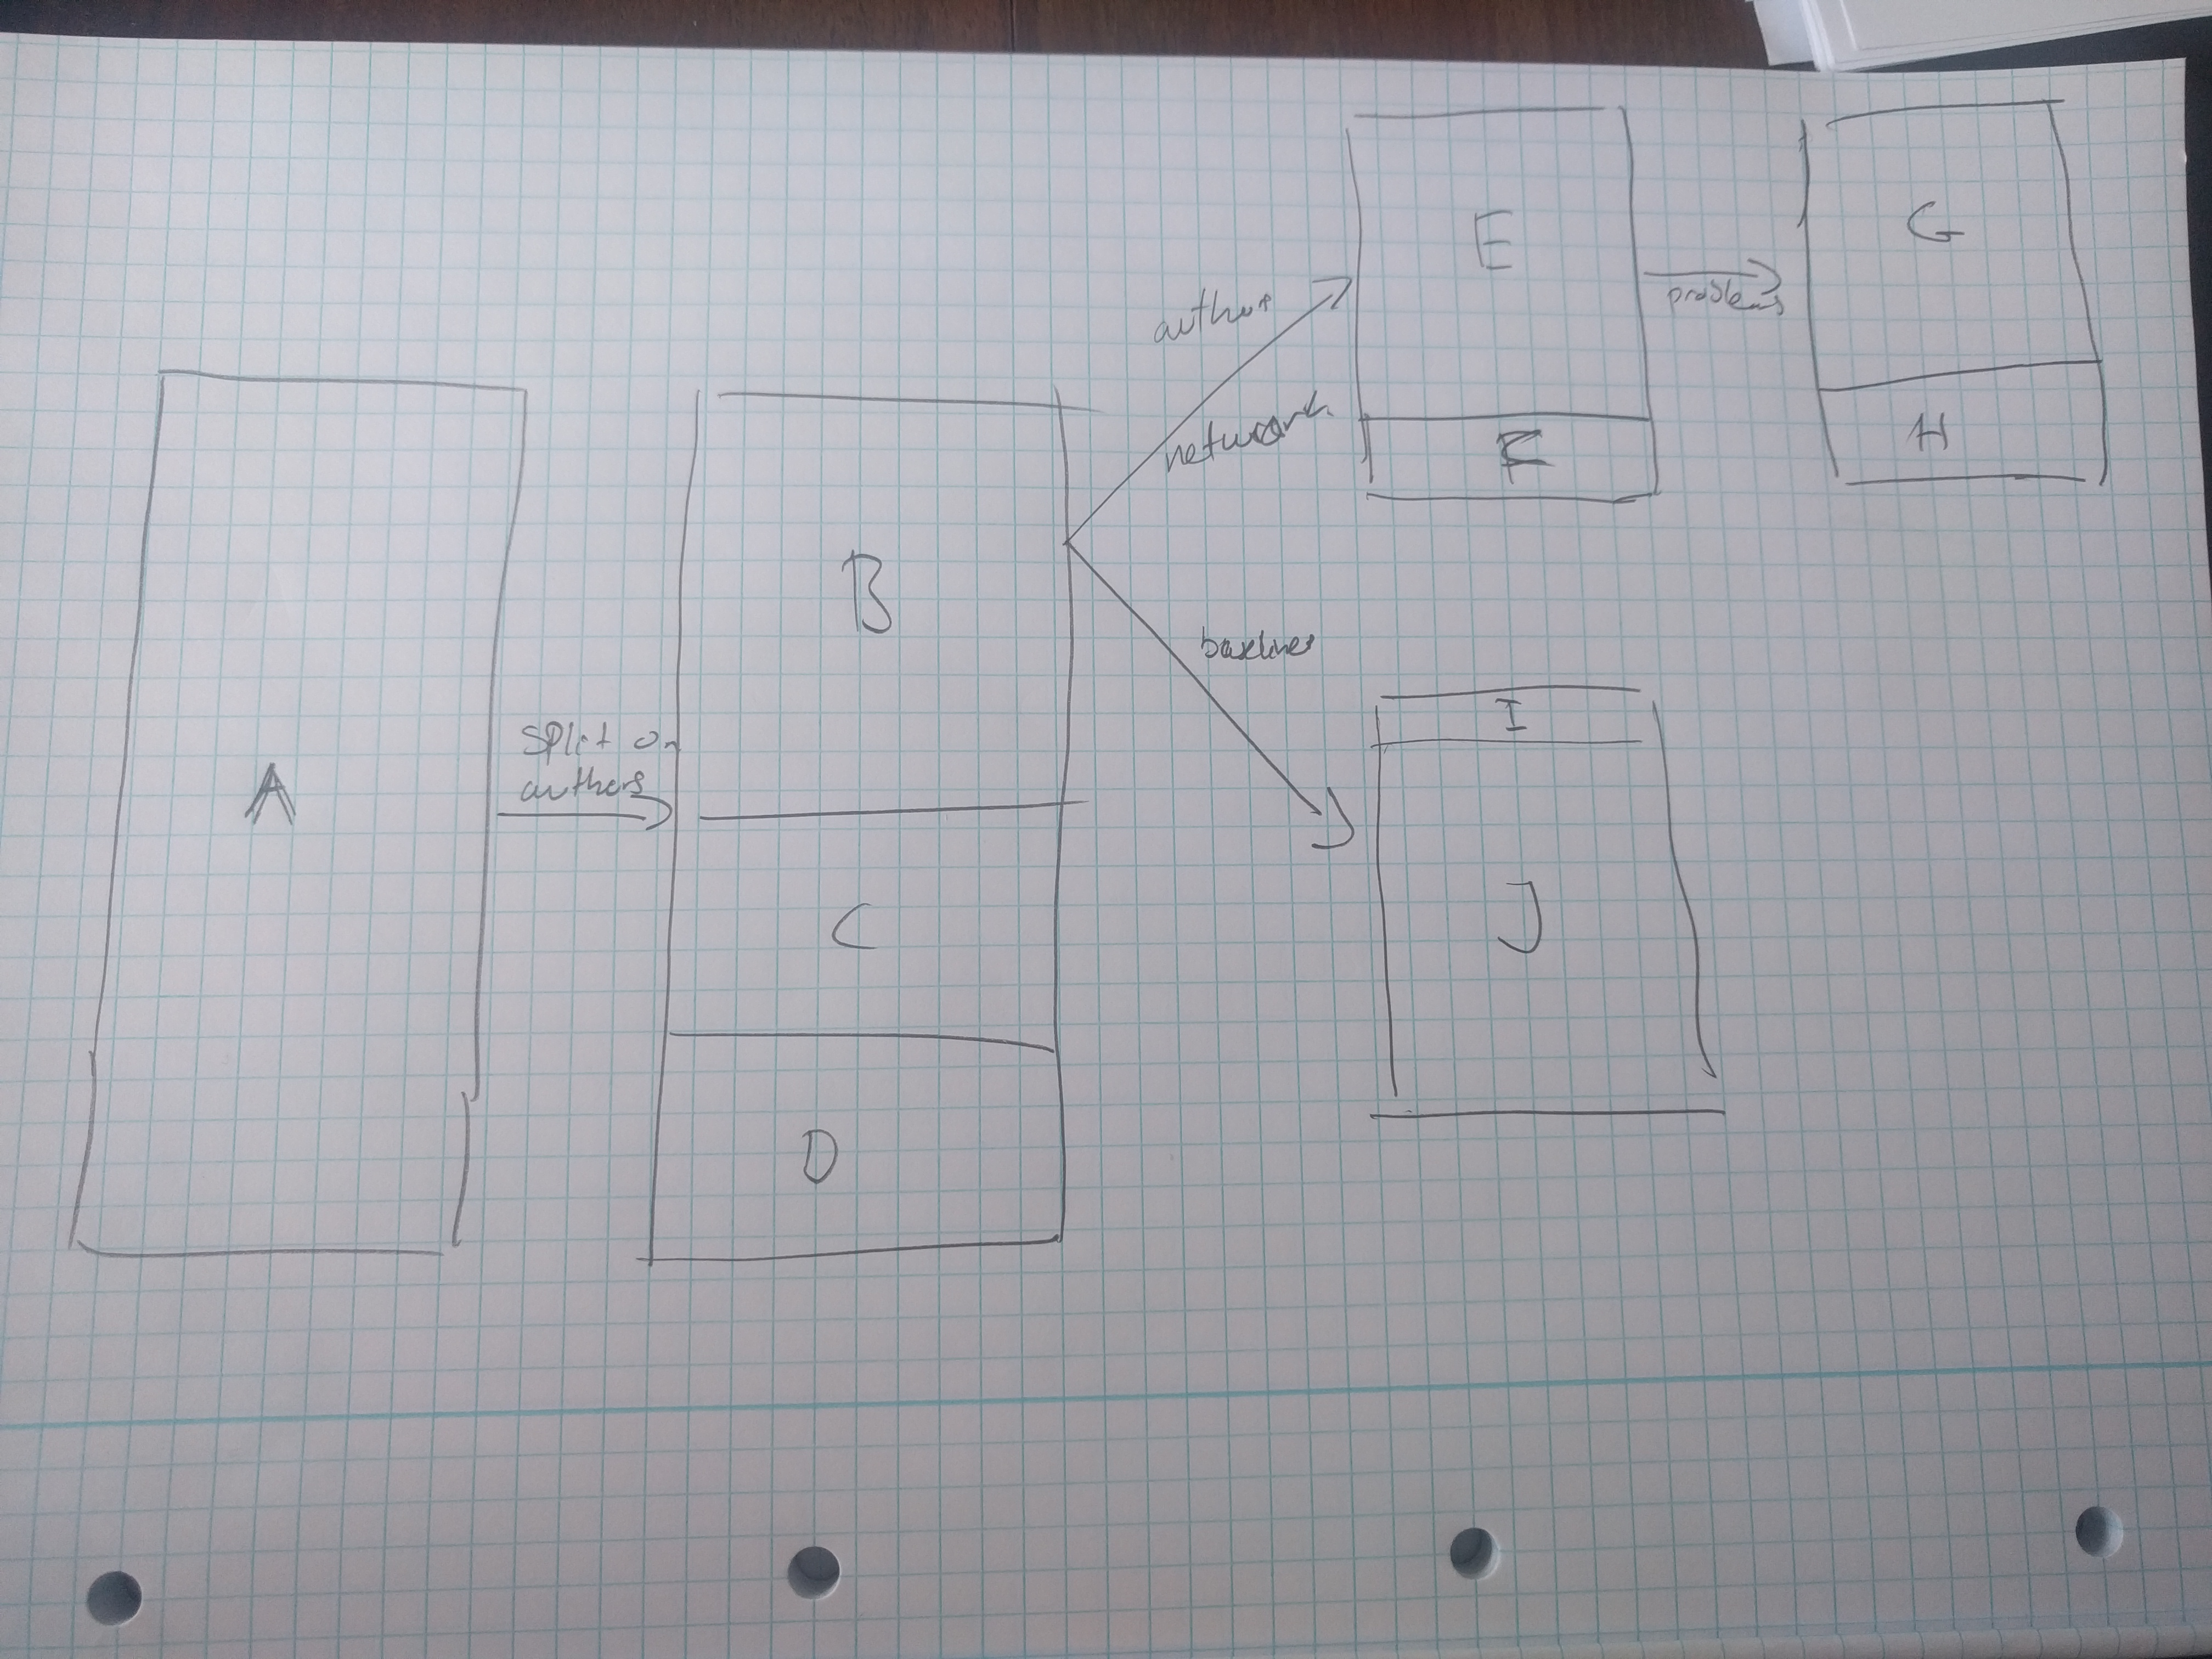
\includegraphics[width=.6\textwidth]{./pictures/data/data_split}
    \caption{Shows how we have split the dataset we are given. The splits are
        performed on the number of authors in each set. That means that all of
        an authors texts are contained in the same dataset. In particular that
        means that the test dataset contains completely unseen authors that has
        not been used in any training and hyper-parameter selection.}
    \label{fig:data_split}
\end{figure}

\begin{description}

    \item[\gls{A}]

        Consists of 10,058 authors and 133,749 texts. This is the original
        dataset we were given by MaCom. The dataset is extracted from high
        school students spanning several different schools.

    \item[\gls{B}]

        Consists of 5,500 authors and 71,451 texts. This dataset is used in
        the training process of the \gls{NN}s, in the hyperparameter selection
        in the baseline methods and as a corpus for extracting statistical
        information about texts and authors.

    \item[\gls{C}]

        Consists of 1,000 authors and 13,130 texts. This dataset is used for
        selecting the best networks we train during the experiments and to give
        an unbiased estimate of network performance on the test dataset.

    \item[\gls{D}]

        Consists of 3,558 authors and 45,824 texts. This dataset is used to
        give an unbiased estimate of the performance of our methods in the real
        world.

    \item[\gls{E}]

        Consists of 3500 authors and 45,251 texts. This dataset is used for
        training our neural networks.

    \item[\gls{F}]

        Consists of 2,000 authors and 26,198 texts. This dataset is used to
        choose hyperparameters for the prediction system.

    \item[\gls{G}]

        Consists of 3,000 authors and 38,773 texts. This is the dataset that are
        used to generate the actual data the networks are trained on. In Section
        \ref{subsec:problem_generation} we describe how we generate individual
        samples to the networks.

    \item[\gls{H}]

        Consists of 500 authors and 6,478 texts. This dataset is used to perform
        early stopping during the training of our neural networks.

    \item[\gls{I}]

        Consists of 100 authors and 1,384 texts. This dataset is used to
        perform feature selection for the \gls{SVM} and Extended Delta
        method. We will describe the feature selection process in Section
        \ref{subsec:baseline_methods}.

    \item[\gls{J}]

        Consists of 5,400 authors and 70,067 texts. This dataset is used to find
        hyperparameters for our baseline methods. We describe the hyperparameter
        selection in Section \ref{subsec:baseline_methods}.

\end{description}


\subsection{Preprocessing}

We apply several preprocessing steps to the dataset. We mainly exclude texts
that are to long or to short or texts that seem like they do not contain valid
text. We base our preprocessing decisions on statistical information extracted
from the B dataset. In the B dataset,

\begin{itemize}

    \item

        Each author has written an average of 13 texts with a standard deviation
        of 4.2. The maximum number of texts per author is 42 and the minimum is
        2,

    \item

        The average character count in a text is 5,517 with a standard deviation
        of 4134 characters. The maximum character count in a text is 338,315 and
        the minimum is 0,

    \item

        The average length of a sentence is 20 words with a standard deviation
        of 25 words. The maximum number of words in a sentence is 6327 and the
        minimum is 0,

    \item

        The average number of sentences per text is 50 sentences with a standard
        deviation of 40 sentences. The maximum number of sentences in a text is
        4401 and the minimum is 0,

    \item

        The average number of unique characters used in a text is 55 with a
        standard deviation of 12. The text with the most unique characters used
        has 219 characters and the minimum is 0,

    \item

        The average number of unique words used in a text is 379 words with a
        standard deviation of 207 words. The maximum unique words used is 13950
        and the minimum is 0.

\end{itemize}

It does not make sense to train networks on a text that contain 0 characters
or a text with a sentence consisting of 6327 words. The text of 0 characters
is clearly a blank hand in and the text with a very long sentence is probably
garbage extracted from a corrupted pdf file. Furthermore some of our methods
require us to hold a text in memory and perform operations on it. Some of the
very long texts caused our programs to crash so we also had to restrict the
length of the texts.

We initially removed the first 200 characters of each text as the beginning of
each text contains metadata such as author name, school of origin, and author
class. We did not discover that we needed to remove the first 200 characters
based on the statistics above. Rather we discovered during our experiments
that the networks were using the metadata to make decisions as described later
in Section \ref{subsubsec:conv_char_nn}. In addition to the 200 characters we
removed initially we also removed texts that had below 200 characters left after
the removal. We did that as we believe they do not provide enough information
about that specific author to be useful. This constraint resulted in 2.49\%
of the texts being removed. Furthermore we applied an upper character count
constraint for computational reasons. We found that limiting the number of
characters to 30.000 gave good results by removing the troublesome, without
affecting the data-quality too much. This constraint resulted in the removal of
0.16\% of the texts being removed. We have illustrated the cutoffs in Figure
\ref{fig:cutoff_thresholds}. There it can be seen that the cutoff points removes
only the outliers and leaves the vast majority of texts.

Since we used some sentence level networks as well, we also chose to limit
the maximum number of sentences. The text with the most sentences also caused
memory problems giving us another reason to limit the number of sentences in a
text. We chose to impose an upper limit of 500 sentences which is well above the
average sentence count. In Figure \ref{fig:cutoff_thresholds} we have shown the
fraction of texts removed by this upper limit. It can be seen that almost no
texts are removed. Specifically 0.35 \textperthousand of the texts were removed.

The last constraint regards the number unique characters in each text. Looking
at the statistics we can see that there is a text containing 219 unique
characters. Such a high unique character count implies that a non-Danish
alphabet might have been used and for that reason that text is not useful for
our purposes. We dealt with the many different unique characters by replacing
all characters with a frequency less than $10^{-5}$ with a special garbage
character. Our neural networks were then supposed to learn that that garbage
character should be ignored. We chose the threshold based on the frequencies
of the Danish characters æ, ø, å, Æ, Ø and Å. We believe that those
characters are important to determining authorship as for example some people
replace the character å with aa and others do not. The frequency of those
characters lie just above the $10^{-5}$ threshold we chose. Additionally we can
see in Figure \ref{fig:cutoff_thresholds} that after the threshold the overall
of frequency of the characters drops dramatically. Which suggests that we chose
a correct threshold.

After applying all of the constraints and taking into account overlap between
them only 2.65 \% of the texts were removed. The amount is negligible amount
compared to the computational and generalization advantages it gives. We also
applied the preprocessing steps to the other datasets meaning that from now on
all datasets has been preprocessed.

\begin{figure}[htb]
    \centering
    \textbf{Data statistics and thresholds}\\
    \begin{minipage}{.5\linewidth}
        \centering
        \subfloat[]{
            \label{subfig:character_frequencies}
            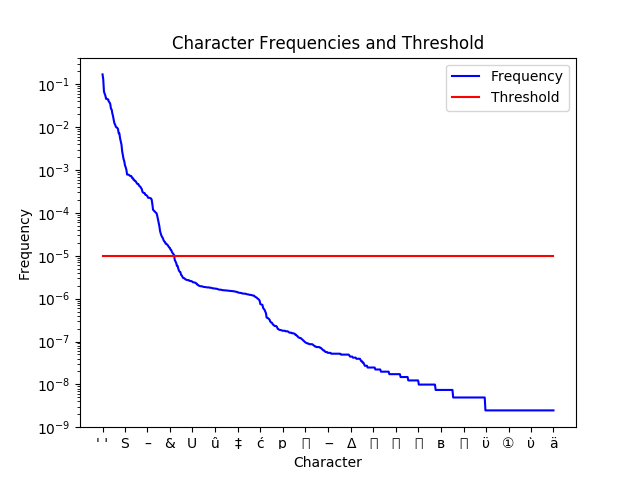
\includegraphics[scale=.5]{./pictures/data/Frequencies}
        }
    \end{minipage}%
    \begin{minipage}{.5\linewidth}
        \centering
        \subfloat[]{
            \label{subfig:sentence_count}
            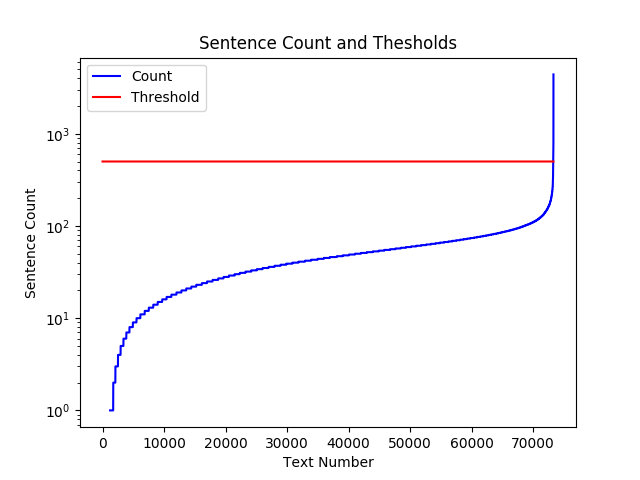
\includegraphics[scale=.5]{./pictures/data/SentenceCount}
        }
    \end{minipage}\par\medskip
    \centering
    \subfloat[]{
        \label{subfig:character_count}
        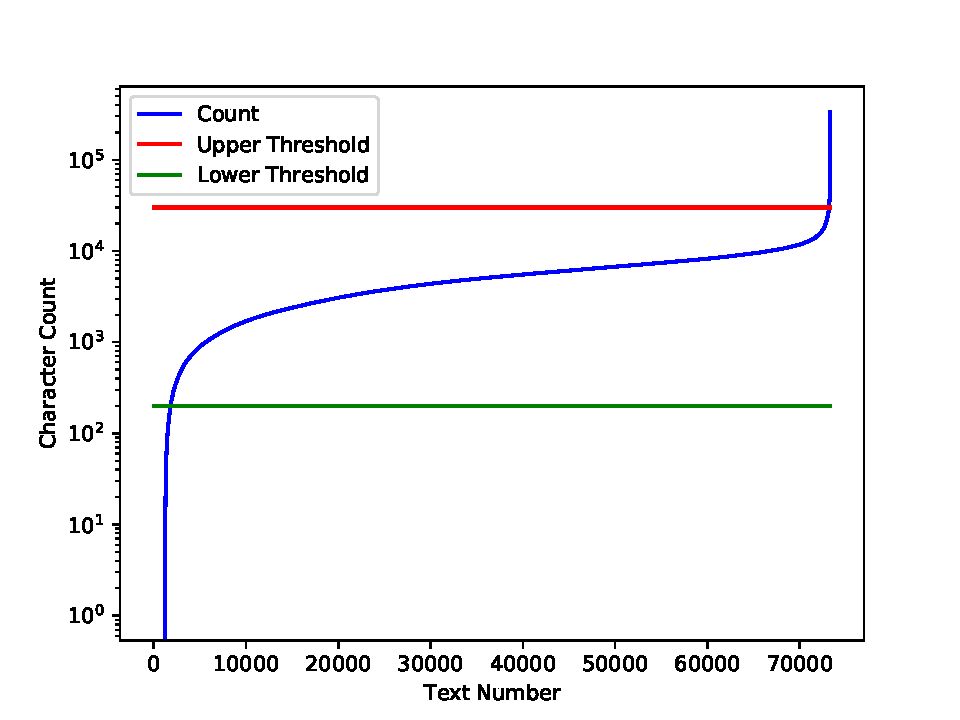
\includegraphics[scale=.5]{./pictures/data/CharacterCount}
    }

    \caption{The different thresholds applied to the during preprocessing. In
        Figure \ref{subfig:character_frequencies} we have shown the thresholds
        we applied to remove the very infrequent characters from the texts. In
        Figure \ref{subfig:sentence_count} we have shown the upper limit we
        placed on sentences. In Figure \ref{subfig:character_count} we have
        shown the upper and lower thresholds we placed on the character count in
        each text.
    }
    \label{fig:cutoff_thresholds}
\end{figure}


\subsection{Neural Network Sample Generation} \label{subsec:problem_generation}

All of the neural networks we trained were Siamese Neural Networks that
compared two texts. We therefore had to generate problem instances that
contained two texts from either the same or different authors and a class
that reflected that. For each author $\alpha$ in the training dataset \gls{G}
we generate all possible combinations of two of the texts in $T_\alpha$ as
positive samples. We also generate the same number of negative samples by
taking a random text in $T_\alpha$ and a random text in $\overline{T_\alpha}$.
This the total number of problems we generate for each
author is $2\frac{\left|T_\alpha\right|!}{2!(\left|T_\alpha\right|-2)!}
= \frac{\left|T_\alpha\right|!}{(\left|T_\alpha\right|-2)!} =
\left|T_\alpha\right| \cdot (\left|T_\alpha\right| - 1) $. The neural
networks were trained on these problem instances. We generated problems in the
same way for the network training validation dataset $H$.
